\chapter{Conclusions and outlook}\label{chap:conclusions}

%TODO brief intro

\section{Conclusions}

%TODO Conclusions

\section{Outlook}

%TODO Outlook

{\color{blue}
Outlook points:	

\begin{itemize}
	\item The $K^2$ surface topology is probably also easily captured using twisted homology/ordinary 1st cohomology. The other two surfaces are more complicated: in the front ($xz$) surface, the chirality change is induced by mirroring across $k_x=0$ (probably can be captured using equivariant cohomology on the surface), while in the $yz$ surface it is induced by a change of projection direction (cannot be captured using equivariant homology, the effective surface BZ is a torus).
	
	\item This description may be easily extendable to a 2D type AIII Klein bottle WSM with chiral symmetry; in this case, 1st cohomology invariants (winding numbers) are dual to twisted 1st homology invariants (Fermi arcs/loops).
	
	\item More elementary systems such as 3D type A with inversion symmetry also exhibit non-orientable EBZs, but in this case the description is complicated by the existence of fixed points (the TRIM).
	
	\item Applicability of this description is probably limited under addition of non-trivial additional bands, e.g. 4-band models incorporating spin and orbital degrees of freedom. The full scope of applicability is somewhat of an open question at this point. (E.g., how well are 2D chiral WSMs described by this homology picture?)
	
	\item Experimental verification in acoustic crystals may be relatively straightforward.
	
	\item Anti-unitary glide symmetry $\implies$ twisted cohomology on $\KS$? %TODO look into anti-unitary space group symm.
\end{itemize}
}

{\color{red}
\section*{Notes}
Concepts explored in early personal notes:
\begin{itemize}
	\item Calculations of (co)homology and semimetal MV sequence for manifolds in $\geq2$ dimensions:
	\begin{itemize}
		\item All compact surfaces without boundary, i.e.\ the surfaces $M_g$ and $N_g$
		
		\item All spaces of the form $M = K^2 \times \T^{d-2}$
	\end{itemize}
	
	\item The map $\Sigma:H^{d-1}(\bigsqcup_{k}S^{d-1})\to H^d(M)$ in the semimetal MV has a clear interpretation in terms of total charge in the (orientable) $d=3$ case. This would provide a clear picture of the total charge cancellation in the orientable case ($H^d(M) = \Z$ in general) vs. the mod 2 charge cancellation in the non-orientable case ($H^d(M) = \Z_2$ in general).
	
	\item However, $\Sigma$ and the other maps in the MV sequence are difficult to interpret in the $\chi\neq 0$ case (maybe even generally for odd dimensions). Taking the oriented case as an example, the MV sequence ends as
	\begin{align*}
		H^{d-1}(M\setminus\Delta)\ \rightarrow\ H^{d-1}\left(\bigsqcup_{k}S^{d-1}\right) \cong \Z^k\ \overset{\Sigma}{\rightarrow}\ H^d(M) \cong \Z
	\end{align*}
	so that the ``charge configuration'' in $\Z^k$ must map to 0 by $\Sigma$ in order to descend from the semimetal, regardless of whether $\chi=0$.
	
	\item This may imply that the Bloch vector field carries more topological information about the total charge than the MV sequence (which makes sense since it generates \emph{all} homology groups of the valence bundle, and all Betti numbers factor into $\chi$). As a concrete example, consider $M=S^2$ with a single puncture of charge $+2$. The punctured sphere is topologically a disc, so that the valence bundle must be trivial, while the Bloch vector field is topologically non-trivial in the sense that it has an index $+2$ singularity. In addition, all relevant $H_n(A)\oplus H_n(B)$ are zero, so that the semimetal MV reduces to the statement that $H_2(S^2)\cong H_1(S^1)$.
	
	\item It may even be the case that the valence bundle cannot be generated from the Bloch vector field in the $d=2$ case; it's probably worth studying the $d\in\set{3,4,5}$ cases (pullback of some universal bundle) to learn more about this. The $d=3$ case should be especially helpful in understanding how the valence bundle arises from the vector field.
	
	\item A complicating factor in the non-orientable case is that the homology groups are different from the cohomology groups, since the torsion moves up one dimension. This makes the homological semimetal MV different from the cohomological one (it's a short exact sequence in $d\geq3$!), and this leads to additional challenges in interpretation.
	
	\item The map $H: \R^3\to\la[su](2),\ \vec{h}\mapsto \vec{h}\cdot\vec{\sigma}$ is an isomorphism of Lie algebras, with the cross product as a Lie bracket on $\R^3$. Still the vector field is discontinuous on a non-orientable manifold, while $H$ is not. This suggests an alternative approach for constructing the valence bundle: consider $h$ as a map $M\to\R^d$ instead of an element of $\vct(M)$, and then pull back the universal bundle along the unit map $\hat{h}:M\setminus\Delta\to S^{d-1}$. That is, we detach $\vec{h}$ from the tangent bundle and consider it a more abstract map. An added ``benefit'' of this is that we lose all coordinate dependence. However, this may also be a downside in the sense that the map will not be subject to the same constraints (Poincaré--Hopf etc.) that the vector field is; for example, $S^2\to\R^2,\ x\mapsto(1,0)$ is a perfectly valid map that would violate the hairy ball theorem as a vector field (and this is a result of being unable to cover $S^2$ by a single chart). At this point the question may become more about which description is more physical in nature, and the non-orientable Weyl point paper\cite{Fonseca-Vaidya_nonorientable} seems to imply there may be more to the $h:M\to\R^3$ story. It also seems to agree better with the intuition of an applied external potential removing all Weyl nodes -- something that's impossible for $\chi\neq0$ if charge corresponds to vector field index. It also explains how the valence bundle can be trivial on the once punctured $S^2$.
	
	\item In light of the previous point, this may be an important observation: every $d$-manifold $M$ with $\chi(M)=0$ admits a nowhere-vanishing vector field (\href{https://math.stackexchange.com/questions/47370/if-a-manifold-m-has-zero-euler-characteristic-there-is-a-non-vanishing-vector-f}{link}). \st{This may imply that the vector field description is equivalent to the map to $\R^d$ in these cases, though one needs to be careful about charts. It would be good to find or write a (dis)proof for something like $\vct(M)\cong\Cinf(M,\R^d)$ (or similar for non-vanishing maps) in this case. Or more specifically:}
	\[
	\st{\big[M\setminus\Delta,S^{d-1}\big] \stackrel{?}{\cong} \Set{\vec{h}\in\vct(M\setminus\Delta) | \text{$\vec{h}$ is non-vanishing}}}
	\]
	Update: I think the real requirement for equivalence is that the base manifold $M$ is parallelisable (i.e.\ has a trivial tangent bundle), since we're essentially using a trivial $\R^d$-bundle in this construction.
	
	\item Any smooth $d$-manifold can be given a CW complex structure with one $d$-cell (\href{https://mathoverflow.net/questions/120799/manifolds-admitting-cw-structure-with-single-n-cell}{link}). On this $d$-cell there is an exact correspondence between vector fields and maps to $\R^d$, since it can be embedded in $\R^d$. What distinguishes the two is how points on the boundary of the $d$-cell are identified with each other; this determines whether the ``vectors'' need to change orientation. To illustrate:\\
	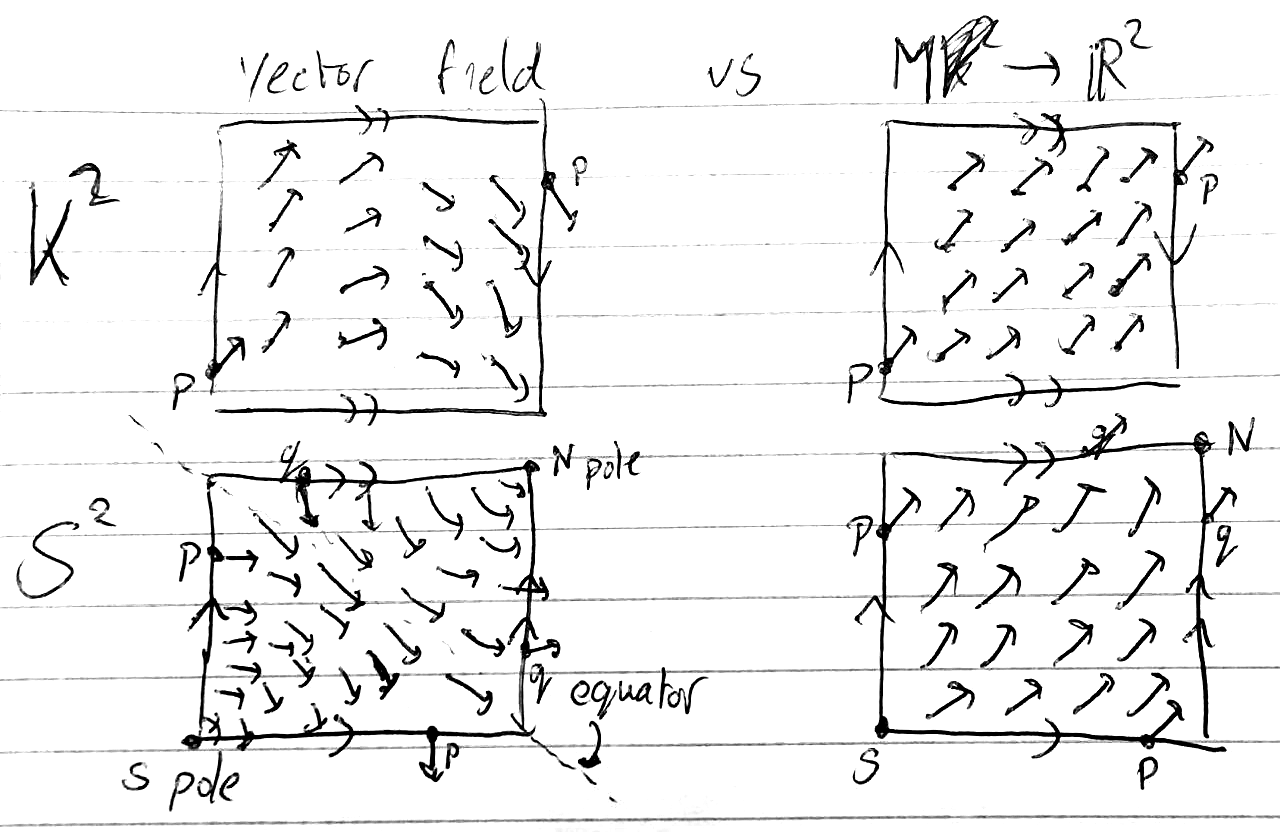
\includegraphics[width=.9\textwidth]{Images/vectorfield-vs-map}
	
	\item On any orientable manifold, the Stokes' theorem argument shows that the total charge must be zero regardless of Euler characteristic:
	\[
	\sum_{\alpha}w(S_\alpha) = \sum_{\alpha}\int_{S_\alpha} c_1(E) = \sum_{\alpha}\int_{S_\alpha}\frac{\Tr\Fc}{2\pi} = \int_{B'} \dd{\frac{\Tr\Fc}{2\pi}} = 0
	\]
	where the last equality holds by the Bianchi identity for the trace. This means the valence bundle cannot be a pullback along a tangent vector field for $\chi\neq0$.
	
	On a non-orientable manifold, this argument doesn't hold since the integral over $B'$ isn't well defined.
	
	\item Total chirality isn't well defined on a non-orientable manifold (at least in odd dimensions, not sure how to interpret even dimensions). Still there is charge cancellation in the form of Fermi arcs etc.; it may take moving to a different homology system to get the full picture, such as homology with local coefficients or equivariant homology. (See e.g. Ref.~\cite{Thiang_equivariant})
	
	\item It may be worth classifying which manifolds are candidates for physical material Brillouin zones; I have a feeling that this might be restricted to those manifolds for which the $n$-torus is a covering space. In this case a full classification of symmetries on the torus (and e.g. their related equivariant homologies) would be sufficient to classify all material topologies. This classification is related to space group symmetries.
\end{itemize}
}  % end red colour